\documentclass{ximera}

\graphicspath{  
{./}
{./whoAreYou/}
{./drawingWithTheTurtle/}
{./bisectionMethod/}
{./circles/}
{./anglesAndRightTriangles/}
{./lawOfSines/}
{./lawOfCosines/}
{./plotter/}
{./staircases/}
{./pitch/}
{./qualityControl/}
{./symmetry/}
{./nGonBlock/}
}


%% page layout
\usepackage[cm,headings]{fullpage}
\raggedright
\setlength\headheight{13.6pt}


%% fonts
\usepackage{euler}

\usepackage{FiraMono}
\renewcommand\familydefault{\ttdefault} 
\usepackage[defaultmathsizes]{mathastext}
\usepackage[htt]{hyphenat}

\usepackage[T1]{fontenc}
\usepackage[scaled=1]{FiraSans}

%\usepackage{wedn}
\usepackage{pbsi} %% Answer font


\usepackage{cancel} %% strike through in pitch/pitch.tex


%% \usepackage{ulem} %% 
%% \renewcommand{\ULthickness}{2pt}% changes underline thickness

\tikzset{>=stealth}

\usepackage{adjustbox}

\setcounter{titlenumber}{-1}

%% journal style
\makeatletter
\newcommand\journalstyle{%
  \def\activitystyle{activity-chapter}
  \def\maketitle{%
    \addtocounter{titlenumber}{1}%
                {\flushleft\small\sffamily\bfseries\@pretitle\par\vspace{-1.5em}}%
                {\flushleft\LARGE\sffamily\bfseries\thetitlenumber\hspace{1em}\@title \par }%
                {\vskip .6em\noindent\textit\theabstract\setcounter{question}{0}\setcounter{sectiontitlenumber}{0}}%
                    \par\vspace{2em}
                    \phantomsection\addcontentsline{toc}{section}{\thetitlenumber\hspace{1em}\textbf{\@title}}%
                     }}
\makeatother



%% thm like environments
\let\question\relax
\let\endquestion\relax

\newtheoremstyle{QuestionStyle}{\topsep}{\topsep}%%% space between body and thm
		{}                      %%% Thm body font
		{}                              %%% Indent amount (empty = no indent)
		{\bfseries}            %%% Thm head font
		{)}                              %%% Punctuation after thm head
		{ }                           %%% Space after thm head
		{\thmnumber{#2}\thmnote{ \bfseries(#3)}}%%% Thm head spec
\theoremstyle{QuestionStyle}
\newtheorem{question}{}



\let\freeResponse\relax
\let\endfreeResponse\relax

%% \newtheoremstyle{ResponseStyle}{\topsep}{\topsep}%%% space between body and thm
%% 		{\wedn\bfseries}                      %%% Thm body font
%% 		{}                              %%% Indent amount (empty = no indent)
%% 		{\wedn\bfseries}            %%% Thm head font
%% 		{}                              %%% Punctuation after thm head
%% 		{3ex}                           %%% Space after thm head
%% 		{\underline{\underline{\thmname{#1}}}}%%% Thm head spec
%% \theoremstyle{ResponseStyle}

\usepackage[tikz]{mdframed}
\mdfdefinestyle{ResponseStyle}{leftmargin=1cm,linecolor=black,roundcorner=5pt,
, font=\bsifamily,}%font=\wedn\bfseries\upshape,}


\ifhandout
\NewEnviron{freeResponse}{}
\else
%\newtheorem{freeResponse}{Response:}
\newenvironment{freeResponse}{\begin{mdframed}[style=ResponseStyle]}{\end{mdframed}}
\fi



%% attempting to automate outcomes.

%% \newwrite\outcomefile
%%   \immediate\openout\outcomefile=\jobname.oc
%% \renewcommand{\outcome}[1]{\edef\theoutcomes{\theoutcomes #1~}%
%% \immediate\write\outcomefile{\unexpanded{\outcome}{#1}}}

%% \newcommand{\outcomelist}{\begin{itemize}\theoutcomes\end{itemize}}

%% \NewEnviron{listOutcomes}{\small\sffamily
%% After answering the following questions, students should be able to:
%% \begin{itemize}
%% \BODY
%% \end{itemize}
%% }
\usepackage[tikz]{mdframed}
\mdfdefinestyle{OutcomeStyle}{leftmargin=2cm,rightmargin=2cm,linecolor=black,roundcorner=5pt,
, font=\small\sffamily,}%font=\wedn\bfseries\upshape,}
\newenvironment{listOutcomes}{\begin{mdframed}[style=OutcomeStyle]After answering the following questions, students should be able to:\begin{itemize}}{\end{itemize}\end{mdframed}}



%% my commands

\newcommand{\snap}{{\bfseries\itshape\textsf{Snap!}}}
\newcommand{\flavor}{\link[\snap]{https://snap.berkeley.edu/}}
\newcommand{\mooculus}{\textsf{\textbf{MOOC}\textnormal{\textsf{ULUS}}}}


\usepackage{tkz-euclide}
\tikzstyle geometryDiagrams=[rounded corners=.5pt,ultra thick,color=black]
\colorlet{penColor}{black} % Color of a curve in a plot



\ifhandout\newcommand{\mynewpage}{\newpage}\else\newcommand{\mynewpage}{}\fi


\author{Jenny Sheldon \and Bart Snapp}


\outcome{}


\title{Groups}

\begin{document}
\begin{abstract}
  Groups are one of the most fundamental objects in modern mathematics.
\end{abstract}
\maketitle

One of the most fundamental notions in all of modern mathematics is
that of a \textit{group}. Sadly, many students never see a group in their
education.

\begin{definition}\index{group}
A \dfn{group} is a set of elements (in our case matrices) which we
will call $\mathcal{G}$ such that: 
\begin{enumerate}
\item There is an associative operation (in our case matrix multiplication).
\item The set is closed under this operation (the product of any two
  matrices in the set is also in the set).
\item There exists an identity $\mat{I}$ in $\mathcal{G}$ such that for all $\mat{M}$ in $\mathcal{G}$, 
\[
\mat{I}\mat{M}=\mat{M}\mat{I} = \mat{M}.
\]
\item For all $M$ in $\mathcal{G}$ there is an inverse $\mat{M}^{-1}$ in $\mathcal{G}$ such that 
\[
\mat{M} \mat{M}^{-1}= \mat{M}^{-1}\mat{M}= \mat{I}.
\]
\end{enumerate}
\end{definition}


\section{Groups of rotations}


Let's see an example of a group. Here we have an equilateral triangle centered at
the origin of the $(x,y)$-plane:
\begin{image}
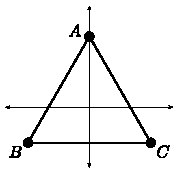
\includegraphics{symTri.pdf}
\end{image}
\begin{question}
The matrix $\mat{R}_{360}$ will rotate this triangle completely
around the origin. What matrix will rotate this triangle one-third of
a complete rotation?
\end{question}

As a gesture of friendship, I'll take this one. One-third of $360$ is
$120$. So we see that $\mat{R}_{120}$ will rotate the triangle one-third
of a full rotation. Do you remember this matrix? Here it is:
\[
\mat{R}_{120} =
\begin{bmatrix}
\frac{-1}{2} & \frac{-\sqrt{3}}{2} & 0\\
\frac{\sqrt{3}}{2} & \frac{-1}{2} & 0\\
0 & 0 & 1
\end{bmatrix}
\]
In spite of the fact that this matrix is messy and that matrix
multiplication is somewhat tedious, you should realize that
\[
\mat{R}_{120}^2 = \mat{R}_{240}\qquad\text{and}\qquad\mat{R}_{120}^3 = \mat{R}_{360}.
\]
Let's put these facts (and a few more) together in what is called a
\textit{group table}\index{group table}. Remember multiplication
tables from elementary school? Well, we're going to make something
like a ``multiplication table'' of rotations. We'll start by listing
the identity and powers of a one-third rotation along the top and
left-hand sides. Setting $\mat{R} = \mat{R}_{120}$ we have:
\[
{
\renewcommand{\arraystretch}{1.2}
\begin{array}{|c||c|c|c|c|c}
\hline 
\circ & \mat{I} & \mat{R} & \mat{R}^2 & \mat{R}^3 & \cdots \\ \hline\hline 
\mat{I} & & & & &  \\ \hline 
\mat{R} & & & & &  \\ \hline 
\mat{R}^2 &  & & & & \\ \hline
\mat{R}^3 &  & & & & \\ \hline
\vdots &  & & & & \\ 
\end{array}}
\]
Since $\mat{R}^3 = \mat{I}$, we need only take our table to
$\mat{R}^2$. In each entry of the table, we write the element we get by multiplying the row heading by the column heading.  (Since matrix multiplication isn't commutative, this is important!)  Now we can write out the complete table:
\[
{
\renewcommand{\arraystretch}{1.2}
\begin{array}{| c || c | c | c |}
\hline 
\circ & \mat{I} & \mat{R} & \mat{R}^2 \\ \hline\hline 
\mat{I} & \mat{I} & \mat{R} & \mat{R}^2 \\ \hline 
\mat{R} & \mat{R} & \mat{R}^2 & \mat{I} \\ \hline 
\mat{R}^2 & \mat{R}^2 & \mat{I} & \mat{R} \\ \hline
\end{array}}
\]
Since matrix multiplication is associative, and we see from the table
that every element has an inverse, we see that 
\[
\{\mat{I}, \mat{R}, \mat{R}^2\}
\]
is a group.

\begin{question} 
What rotation matrices would we use when working with a square?  A
pentagon?  A hexagon?
\end{question}



\section{Groups of reflections}

Let's see another group. Again consider an equilateral triangle.  This
time we are interested in the three lines of reflection that preserve
this triangle:
\begin{image}
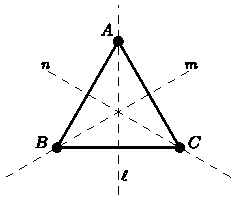
\includegraphics{symTriRef.pdf}
\end{image}

\begin{question}
Suppose that the triangle above is centered at the origin of the
$(x,y)$-plane. What are equations for $\l$, $m$,
and $n$?
\end{question}


The easiest of the reflections above is the reflection over
$\mat{F}_{\l}$.
\begin{image}
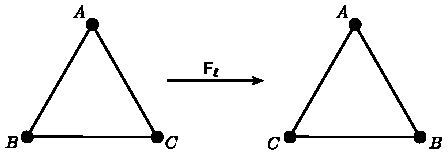
\includegraphics{symTriRef1.pdf}
\end{image}
We'll start our group table off with just two elements: $\mat{I}$ and
$\mat{F}=\mat{F}_{\l}$.

\[
\begin{array}{| c || c | c |}\hline
\circ & \mat{I} & \mat{F} \\ \hline\hline
\mat{I} & \mat{I} & \mat{F} \\\hline
\mat{F} & \mat{F} & \mat{I} \\ \hline
\end{array}
\]

Notice that when we apply $\mat{F}$ twice we're right back where we
started. Hence, $\mat{F} \mat{F} = \mat{I}$. Since matrix
multiplication is associative, we see that
\[
\{ \mat{I}, \mat{F} \}
\]
forms a group. Specifically this is a group of reflections of the
triangle.

\begin{question} 
Above we used $\mat{F}_\l$. What would happen if we used $\mat{F}_m$
or $\mat{F}_n$? Also, what are the equations for the lines of symmetry
of the square centered at the origin?
\end{question}

\end{document}
